\section{Figures and Captions}\label{sec:figs}


Figure and table captions should be centered if less than one line
(Figure~\ref{fig:exampleFig1}), otherwise justified and indented by 0.8cm on
both margins, as shown in Figure~\ref{fig:exampleFig2}. The caption font must
be Helvetica, 10 point, boldface, with 6 points of space before and after each
caption.

\begin{figure}[ht]
	\centering
	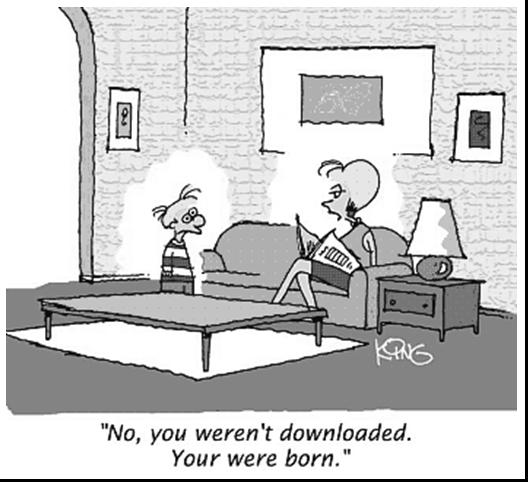
\includegraphics[width=.5\textwidth]{./images/fig1.jpg}
	\caption{A typical figure}
	\label{fig:exampleFig1}
\end{figure}

\begin{figure}[ht]
	\centering
	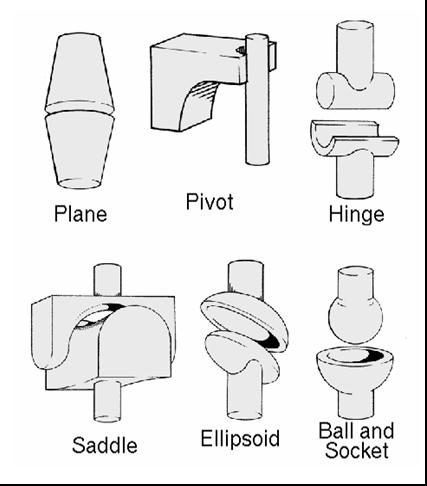
\includegraphics[width=.3\textwidth]{./images/fig2.jpg}
	\caption{This figure is an example of a figure caption taking more than one
		line and justified considering margins mentioned in Section~\ref{sec:figs}.}
	\label{fig:exampleFig2}
\end{figure}

In tables, try to avoid the use of colored or shaded backgrounds, and avoid
thick, doubled, or unnecessary framing lines. When reporting empirical data,
do not use more decimal digits than warranted by their precision and
reproducibility. Table caption must be placed before the table (see Table 1)
and the font used must also be Helvetica, 10 point, boldface, with 6 points of
space before and after each caption.

\begin{table}[ht]
	\centering
	\caption{Variables to be considered on the evaluation of interaction
		techniques}
	\label{tab:exTable1}
	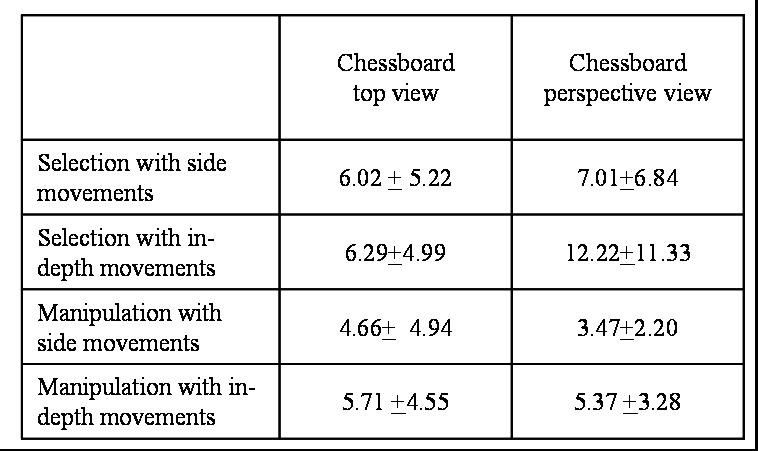
\includegraphics[width=.7\textwidth]{./images/table.jpg}
\end{table}